\subsection{Fixed-Target Posterior Assessment}
\label{sec:supp-mti-posterior-assessment}

The full computation study uses the \MTIFullSimulations{} simulation samples
and \MTIFullApplications{} application training partitions evaluated in this
paper. Each chain holds the sample's ECM-selected \(q,\delta\) fixed, with
\(\omega_{\mathrm R}=1\), zero Gaussian root-prior means, and
\(\lambda=10^{-4}\). Four independently seeded marginal
slice-within-Gibbs chains use 2000 burn-in and 4000 retained cycles, giving
\MTIFullChains{} chains. These calculations sample the generalized
posterior in Section~\ref{sec:supp-mti-ecm}; the content and
tilt search remains the recorded ECM selection rule.

Sorting each draw gives lower and upper endpoints. Their posterior means
define the interval \(I_{\mathrm G}=[\bar l,\bar u]\), with
\(\bar l=\E\{\min(a,b)\mid D_n,q,\delta\}\) and
\(\bar u=\E\{\max(a,b)\mid D_n,q,\delta\}\).
Its width equals the posterior mean of \(|b-a|\).
The sensitivity calculation instead uses the two endpoint medians. The
difference of these medians generally differs from the posterior median
of width. Both summaries condition on the selected fitted content and tilt.

All \MTIFullDatasets{} samples met the preferred recorded criteria:
\(\widehat R\le1.01\), bulk and tail effective sample sizes at least 400,
and mean Monte Carlo error at most 5\% of posterior standard deviation
\citep{VehtariEtAl2021Rhat}. The largest \(\widehat R\) was
\MTIFullRhat{}; the smallest bulk and tail effective sample sizes were
approximately \MTIFullBulkESS{} and \MTIFullTailESS{}.
The largest mean-MCSE/posterior-SD ratio was \MTIFullMaximumMCSE\%.
These checks include both ordered endpoints, width, and midpoint.
No additional sampling was required by the prespecified practical criteria.
All primary means, medians, and credible endpoints also met the separate
1\%-of-posterior-median-width reporting resolution in \MTIFullPrecision{}
samples. The remaining \MTIFullPrecisionOther{} retain their
quantity-specific Monte Carlo errors. This additional resolution measures
reporting precision separately from the mixing diagnostics.

The simulation samples include \MTIFullInterior{} empirical interior,
\MTIFullLimiting{} limiting, and \MTIFullOutside{} outside-range tilts,
using the outward loss rates defined above. These empirical classifications
describe the observed loss surface. At a limiting tilt, an endpoint can
move beyond the data with little loss change, allowing the root prior to
govern substantial posterior dispersion. Outside the empirical range,
outward movement can reduce the unpenalized loss; the Gaussian penalty
retains a proper posterior. This explains why substantial width uncertainty
can remain even in large samples and with well-mixed chains.

\paragraph{Supporting numerical comparisons.}
The earlier assessment used 360 simulation samples, ten application
partitions, and 86 additional extreme-target examples. These 456 cases
overlap the full study. Its separately minimized penalized-loss references
attained relative objective bounds below \(5\times10^{-13}\).
The finite ECM objective gap exceeded \(10^{-4}\) in 96 of those samples,
predominantly at outside-range tilts. These references assess optimization
accuracy of the specified finite calculation. The tolerance comparisons
retain the original ECM intervals.

The original Gaussian/GIG sampler was assessed on a smaller subset.
Among its 20 sample sets meeting the original diagnostic criteria, 77 of
80 matched posterior means were within twice the combined Monte Carlo
standard error of the marginal-sampler estimate; the largest standardized
difference was 2.47. The independently seeded full-study marginal chains
also provide a check against the earlier marginal calculation: of
\MTIFullAgreementCount{} matched means, \MTIFullAgreementTwo{} are within
twice combined MCSE and \MTIFullAgreementThree{} within three times combined
MCSE. The largest absolute standardized difference is
\MTIFullAgreementMaximum{}. These are repeated computational comparisons
on the same data and targets.

Earlier prior sensitivity calculations reweighted the 456-example draws
to Gaussian root variances one half and one tenth of the original value.
They show substantial prior influence in many limiting-tilt examples;
estimates with inadequate importance overlap or excessive Monte Carlo
error remain flagged. Those calculations retain their smaller study scope.
The full study adds the complete empirical-tilt counts and the same-sample
width/content comparisons below.

\begin{figure}[p]
\centering
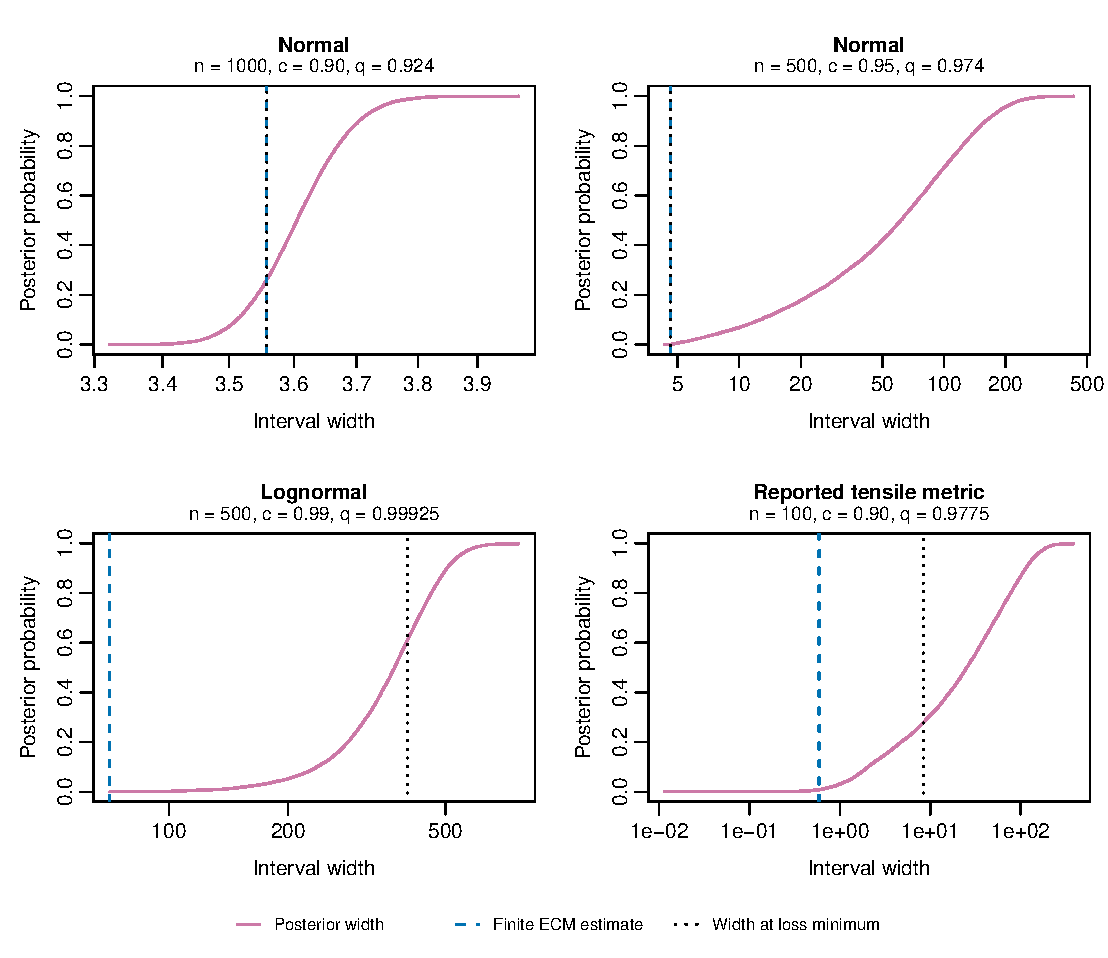
\includegraphics[width=\textwidth]{figures/generated/figS_mti_full_fixed_target_width.pdf}
\caption{\textbf{Posterior width uncertainty at fixed fitted content and tilt.}
The four examples were specified in the earlier computation assessment.
Curves summarize empirical cumulative probabilities of width from the four
full-study chains. Vertical lines mark the finite ECM width and the width
at a separately minimized value of the same penalized loss; coincident
lines indicate agreement of those widths. Each panel uses identical data,
fitted content, tilt, learning rate, and priors for these comparisons.
The panels have separate logarithmic width axes in response units.
Posterior dispersion and finite ECM optimization accuracy are assessed
separately from repeated-sampling content attainment.}
\label{fig:supp-mti-posterior-width}
\end{figure}

\begin{figure}[p]
\centering
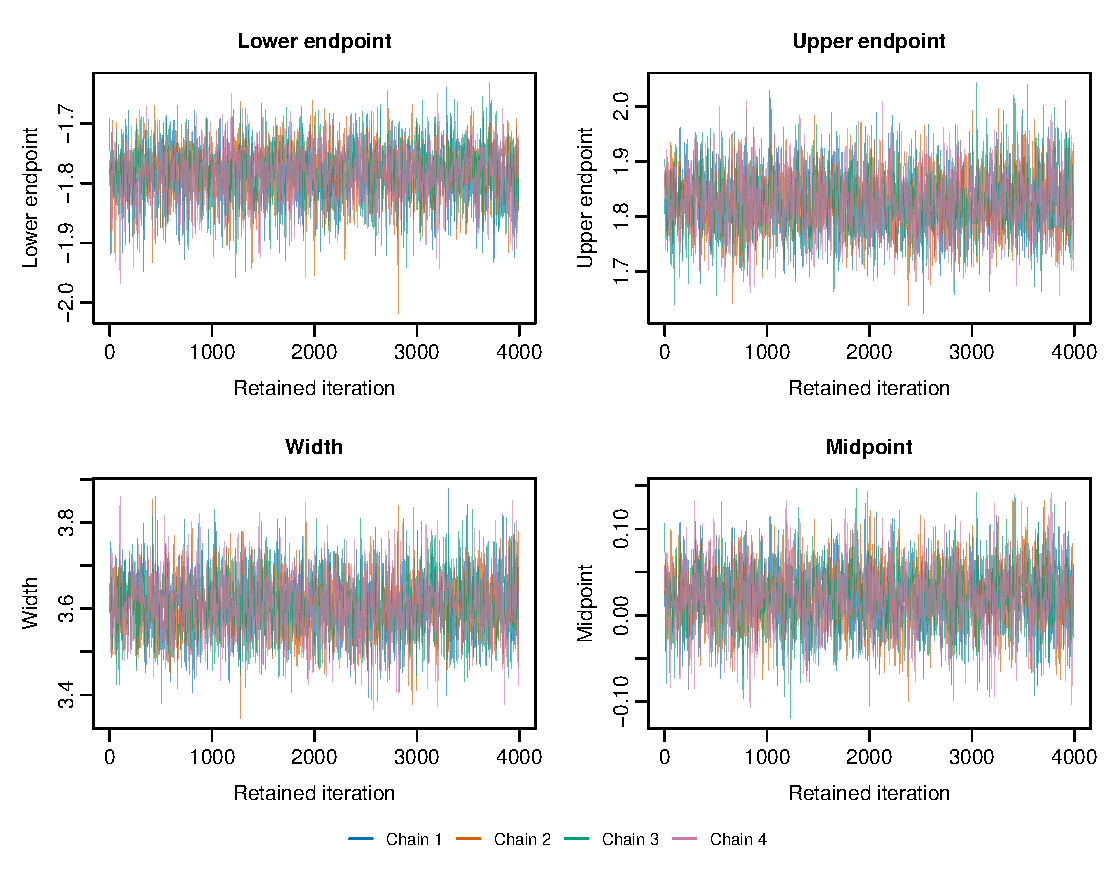
\includegraphics[width=\textwidth]{figures/generated/figS_mti_full_trace.pdf}
\caption{\textbf{Retained root-posterior traces for the prespecified Normal example.}
The sample has \(n=1000\), requested content \(c=0.90\), and fitted content
\(q=0.924\). Colors identify the four chains. Every fourth retained draw
is displayed for clarity; posterior summaries and diagnostics use all
4000 retained draws per chain. The endpoints, width, and midpoint are
derived from the same ordered root pairs.}
\label{fig:supp-mti-full-trace}
\end{figure}

\begin{figure}[p]
\centering
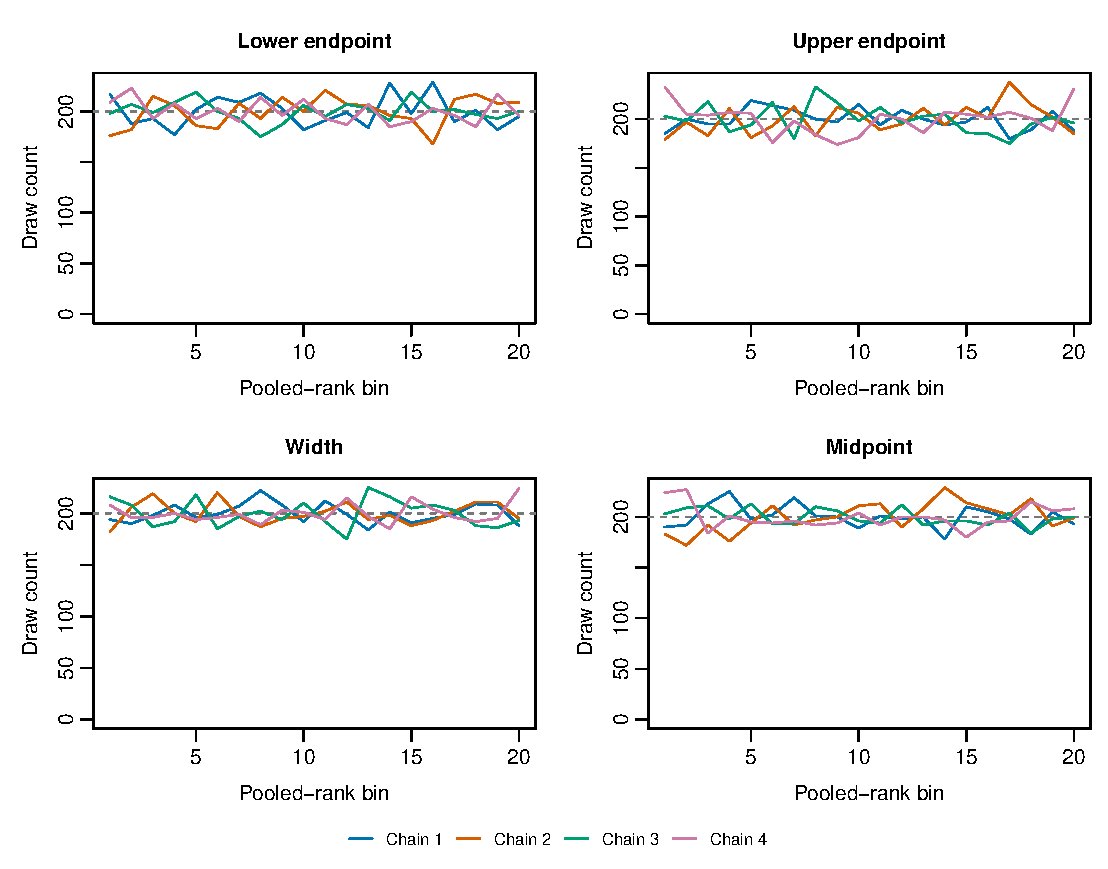
\includegraphics[width=\textwidth]{figures/generated/figS_mti_full_ranks.pdf}
\caption{\textbf{Pooled-rank counts for the Normal example in
Figure~\ref{fig:supp-mti-full-trace}.} Each panel pools all 16,000 retained
values of one quantity, divides their ranks into 20 bins, and shows the
counts contributed by each chain. The dashed line is the equal-count
reference. These graphical comparisons accompany the numerical
multi-chain diagnostics.}
\label{fig:supp-mti-full-ranks}
\end{figure}
